\section{Introduction to downfolding the many electron problem}

In multiscale modeling of many-particle systems, the effective Hamiltonian (or Lagrangian) is one of the most core concepts. 
The effective Hamiltonian dictates the behavior of the system on a coarse-grained level, where `sub-grid' effects are folded into the parameters and form of the effective Hamiltonian. 
Many concepts in condensed matter physics can be viewed as statements about the behavior of the effective Hamiltonian. 
In particular, identification of `strongly correlated' materials as materials where band theory is not an accurate representation of the systems is a statement about effective Hamiltonians.
Effective Hamiltonians at different length scales also form the basis of the renormalization group~\cite{Wilson}.
A major goal in condensed matter physics is to determine what effective Hamiltonians apply to different physical situations, in particular quantum effective Hamiltonians, which lead to large-scale emergent quantum behavior. 

The dominant effective model for quantum particles in condensed systems is band structure, and for metals, Fermi liquid theory. 
However, a major challenge is how this paradigm should be altered when it is no longer a good description of the physical system.
Examples of these include the high-T$_c$ cuprates and other transition metal oxides, which do not appear to be well-described by these simple effective Hamiltonians. 
For these systems, many models have been proposed, such as the Hubbard~\cite{Hubbard1963}, Kanamori~\cite{Kanamori1963}, $t$-$J$~\cite{tJSpalek} and Heisenberg models.
While these models have been extensively studied analytically and numerically, and have significantly enhanced our understanding of the physics of correlated electrons, their effectiveness for describing a real complex system of interest is often unclear. 
At the same time, more complex effective models can be commensurately more difficult to solve,  so one would like to also find an accurate effective model that is tractable. 

%\begin{figure}
%\centering
%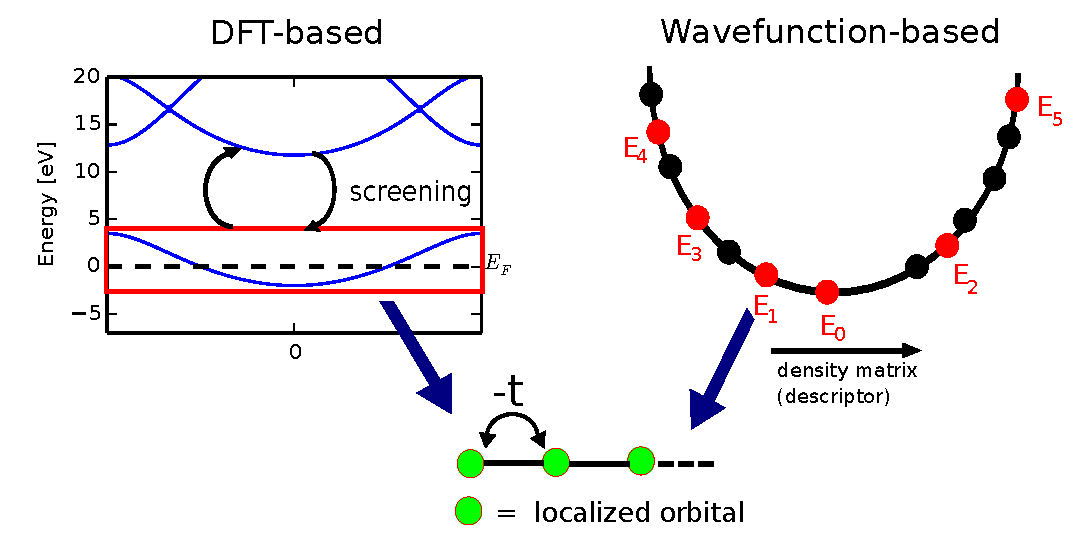
\includegraphics[width=1\linewidth]{./Figures/figure1.eps}
%\caption{Schematics for downfolding a simple ab-initio system (here the hydrogen chain) in DFT based methods (left) and the wave function based DMD (right). 
%Localized one particle functions are constructed in both methods and serve as the one body space for the model Hamiltonian. 
%The DFT based methods use Kohn Sham orbitals and screening models to estimate the interactions. 
%DMD uses a database of low energy all electron many-body wave functions ($\psi_i$). 
%This ``low energy basin" (shown abstractly in the space of descriptors) need not consist of exact eigenstates ($E_i$).\lucas{The energy should be a linear function of the density matrix!}}
%\label{fig:lowenergybasin_schematic}
%\end{figure}	

To address the need for a link between {\it ab-initio} electron-level models and larger scale models, downfolding has most commonly been carried out using approaches based on density functional theory (DFT). 
The kinetic part\BDB{kinetic part of what?}is obtained from a standard DFT calculation which is projected onto localized Wannier functions and gives an estimate of the effective hoppings of the lattice model based on Kohn-Sham band structure calculations~\cite{Pavirini}. 
Then, to estimate the interactions, one assumes a model of screening of the Coulomb interactions based on constrained DFT, RPA, or some other methods. 
Since effects of interactions between the orbitals of interest have already been accounted for by DFT, a double counting correction is required to obtain the final downfolded Hamiltonian. 
The approach has been developed and widely applied~\cite{Pavirini, Dasgupta, Aryasetiawan2004, Jeschke2013}; but remains an active area of research~\cite{Haule_doublecounting}.
There are other downfolding approaches that include the traditional Lowdin method, coupled to a stochastic approach~\cite{Tenno,Zhou_Ceperley} and the related method of canonical transformations~\cite{White_CT, Yanai_CT}. 
While they have many advantages, it is typically not possible to know if a given model {\it ansatz} was a good guess or not, and it is very rare for a technique to provide an estimate of the quality of the resultant model. 

The situation described above stands in contrast to the derivation of effective classical models. 
For concreteness, let us discuss classical force fields computed from {\it ab initio} electronic structure calculations. 
Typically, a data set is generated using an {\it ab initio} calculation in which the positions of the atoms and molecules are varied, creating a set of positions and energies. 
The parameters in the force field {\it ansatz} are varied to obtain a best-fit classical model.
Then, using standard statistical tools, it is possible to assess how well the fit reproduces the {\it ab initio} data within the calculation, without appealing to experiment. 
While translating that error to error in properties is not a trivial task\lucas{citations}, this approach has the important advantage that in the limit of a high quality fit and high quality {\it ab initio} results, the resultant model is predictive.

Na\"ively, one might think to reconcile the fitting approach used in classical force fields with quantum models by matching eigenstates between a quantum model and {\it ab initio} systems, varying the model parameters until the eigenstates match~\cite{Wagner2013}. 
However, this strategy does not work well in practice because it is often not possible to obtain exact eigenstates for either the model or the {\it ab initio} system.
To resolve this, we develop a general theory for generating effective quantum models that is exact when the wave functions are sampled from the manifold of low-energy states. 
Because this method is based on fitting the energy functional, 
We will show the practical application of this theory using both exact solutions and {\it ab-initio} quantum Monte Carlo (QMC) to derive several different quantum models.


The endeavor we pursue here is to develop a multi-scale approach in which the effective interactions between quasiparticles (such as dressed electrons) are determined after an \textit{ab-initio} simulation (but not necessarily exact solution) of the continuum Schroedinger equation involving all the electrons. 
The method uses reduced density matrices (RDMs) of low-energy states, not necessarily eigenstates, 
to cast downfolding as a fitting problem. 
We thus call it density matrix downfolding (DMD).
In this paper, these states will typically be generated using QMC techniques [either variational Monte Carlo (VMC) or diffusion Monte Carlo (DMC)] to come close to the low energy manifold.
The remainder of the paper is organized as follows:
\begin{itemize} 
\item 	In Section 2, we clarify and make precise what it means to downfold 
a many-electron problem to a few-electron problem. We recast the problem into minimization 
of a cost function that needs to be optimized to connect the many and few body problems. We further 
these notions both in terms of physical as well as information science descriptions, which allows us to connect to compression algorithms in the machine learning literature. 
\item Section 3 discusses several representative examples where we consider multiband lattice models 
and ab-initio systems to downfold to a simpler lattice model. 
\item In Section 4, we discuss future prospects of applications of the DMD method, ongoing challenges 
and clear avenues for methodological improvements. 
\end{itemize}


